\section{Décodeur 7 segment}
\subsection{Introduction}
Nous allons commencer par une prise en main de logisim en réalisant un décodeur 7 segments. Ce type d'afficheur est un grand classique en ce qui concerne l'affichage de caractères hexadécimaux.

Le principe de cet afficheur est très simple, En allumant plusieurs segments en même temps nous allons pouvoir représenter les caractères suivants :
0,1,2,3,4,5,6,7,8,9,A,B,C,D,E,F.

\begin{figure}
        \makebox[\textwidth]{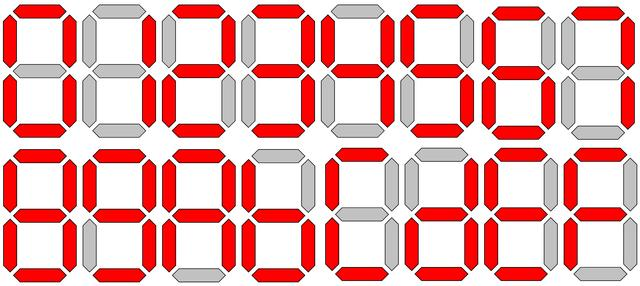
\includegraphics[width=15cm]{pictures/7seg.jpg}}
	\caption{Un affichage hexadécimal par 7 segments. Merci à @Skywodd - https://www.carnetdumaker.net/}
\end{figure}

\subsubsection{meow}
miaounyanmeowmjau

